
%%% Preamble
\documentclass[paper=a4, fontsize=11pt]{scrartcl}
\usepackage[utf8x]{inputenc}
%\usepackage[T1]{fontenc}
\usepackage[brazilian]{babel}															% English language/hyphenation
\usepackage[protrusion=true,expansion=true]{microtype}	
\usepackage{amsmath,amsfonts,amsthm} % Math packages
\usepackage{graphicx}	
\usepackage{url}
\usepackage{caption}
\usepackage{subcaption}
\usepackage{float}
\floatplacement{figure}{H}


%%% Custom sectioning
\usepackage{sectsty}
\allsectionsfont{\centering \normalfont\scshape}


%%% Custom headers/footers (fancyhdr package)
\usepackage{fancyhdr}
\pagestyle{fancyplain}
\fancyhead{}											% No page header
\fancyfoot[L]{}											% Empty 
\fancyfoot[C]{}											% Empty
\fancyfoot[R]{\thepage}									% Pagenumbering
\renewcommand{\headrulewidth}{0pt}			% Remove header underlines
\renewcommand{\footrulewidth}{0pt}				% Remove footer underlines
\setlength{\headheight}{13.6pt}

\graphicspath{{img/}}

%%% Equation and float numbering
\numberwithin{equation}{section}		% Equationnumbering: section.eq#
\numberwithin{figure}{section}			% Figurenumbering: section.fig#
\numberwithin{table}{section}				% Tablenumbering: section.tab#


%%% Maketitle metadata
\newcommand{\horrule}[1]{\rule{\linewidth}{#1}} 	% Horizontal rule

\title{
		%\vspace{-1in} 	
		\usefont{OT1}{bch}{b}{n}
		\normalfont \normalsize \textsc{UFMG - Departamento de Ciência da Computação} \\ [25pt]
		\horrule{0.5pt} \\[0.4cm]
		\huge Indexador de páginas da Web \\
		\horrule{2pt} \\[0.5cm]
}
\author{
		\normalfont 								\normalsize
        Gabriel Miranda Pedrosa\\[-3pt]		\normalsize
        %\today
}
%\date{}


%%% Begin document
\begin{document}
\maketitle
\section{Introdução}
A recuperação de informação é uma tarefa importante quando tratamos de coleções de dados. Quando a quantidade de dados é grande, boas estratégias devem ser adotadas para que as buscas possam ser feitas em tempo hábil. Os dados passam a ser organizados na forma dos chamados índices invertidos de documento, no qual uma palavra referencia os documentos nos quais aparece, em vez do contrário. 

A tarefa do segundo trabalho prático da disciplina de Recuperação da informação é implementar um indexador de páginas Web. O objetivo é realizar a análise das páginas HTML, extrair os termos indexáveis e gerar o índice invertido usando memória externa.

\section{O indexador}
\subsection{Extração dos termos}
A criação do índice começa com a análise das páginas Web da coleção. Essa tarefa é auxiliada pela biblioteca htmlcxx~\footnote{Disponível em: \url{http://htmlcxx.sourceforge.net}} que gera árvores de análise sintática do HTML da página e facilita a extração dos termos indexáveis. Termos extraídos são normalizados e reescritos em caixa baixa.

\subsection{Geração das tuplas}
A indexação continua iterando sobre os termos indexáveis de cada página (documento) e armazenando tuplas de códigos que referenciam o termo, o documento, a frequência daquele termo no documento e as posições onde aparece. Para limitar o uso de memória, pré-determinamos o número de tuplas de termos que podem ser armazenadas em memória principal. Quando essa quantidade é atingida, o conjunto de tuplas é ordenado e armazenado em memória secundária. Este limite é calculado considerando que a tupla ocupa 212B, que é o quanto um termo que aparece em 50 posições de um documento ocuparia em memória.

\subsection{Ordenação externa}
Os arquivos de tuplas ordenadas são mesclados através do algoritmo heapsort multi-way, respeitando o limite do número de tuplas estabelecido. O algoritmo é executado até que sobre um arquivo somente, com todas as tuplas da coleção. Este arquivo, somado dos arquivos que relacionam termos e URLs de páginas com seus respectivos códigos, forma o índice de documentos invertido. A mesclagem dos arquivos não é feita in-place, o que significa que a mesclagem de um arquivo A com o arquivo B gera um terceiro arquivo C com o conteúdo de A e B.

\section{O Buscador}
Como parte da tarefa, um buscador que utilizasse o índice gerado deveria ser implementado. A busca recuperava a lista de documentos que cada um dos termos da consulta aparecia e retornava a interseção entre todas as listas. A interseção era calculada ordenando as listas pelo tamanho delas. A menor lista era tomada como referência e a presença de seus elementos nas outras listas era verificada, de forma que somente eram retornados documentos que apareciam nas listas de todos os termos da busca.

\section{Análise de complexidade}
\subsection{Tempo}
As tarefas que mais demandam tempo na indexação é a geração de termos indexáveis e a ordenação externa. A primeira gera uma árvore sintática que é usada para navegar pelo documento em busca dos termos. Considerando que a construção é feita em tempo linear, a extração de termos é feita em $O(C)$, em que $L$ é o tamanho do documento em número de caracteres. A segunda tarefa executa um heapsort multi-way que tem ordem de complexidade $O(T log_{W} T)$, em que $T$ indica o número de tuplas a serem ordenadas e $W$ o número de tuplas que vão para a memória principal.

\subsection{Espaço}
Os módulos mais custosos em espaço são o vocabulário e as tuplas armazenadas em memória principal. O vocabulário ocupa espaço $O(V)$, em que $V$ indica o tamanho do vocabulário. Uma tupla armazena também as posições onde aparece no documento. Por isso, a complexidade média de espaço é da ordem $O(P)$, onde $P$ indica a frequência média de termos em documentos da coleção.

\section{Experimentos}
Para avaliar o desempenho do indexador implementado, foram realizados testes para analisar a resposta quando variamos o número de tuplas disponíveis em memória principal e o número de documentos para indexar. Foi usada uma coleção de 5GB, com 8608 termos e 21924 documentos, segundo o índice gerado pelo indexador. A coleção corresponde aos 10 primeiros documentos da coleção completa disponibilizada em sala. O computador utilizado para os experimentos foi:
\begin{itemize}
  \item 1.4 GHz Intel Core i5
  \item 4 GB 1600 MHz DDR3
  \item OS X El Capitan
  \item SSD 128GB
\end{itemize}

\subsection{Tamanho da coleção}
Fixando o tamanho da memória disponível em 200 megabytes, o tamanho da coleção foi variado em 2,5GB e 4,5GB. O resultado de tempo de indexação pode ser observado no gráfico~\ref{fig:tamanho}. É possível validar a ideia de que quanto maior a coleção, mais tempo o indexador leva.

\begin{figure}
  \caption{Tempo de indexação em função do tamanho da coleção}
  \label{fig:tamanho}
  \centering
    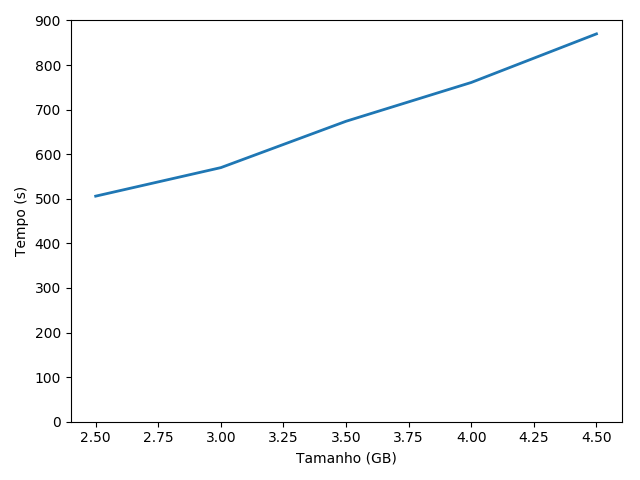
\includegraphics[width=0.6\textwidth]{tamanho}
\end{figure}

\subsection{Tuplas}
Foi passada a memória disponível como parâmetro variando entre 20, 40, 60, 80 e 100 megabytes. O tamanho da coleção foi fixado em 2,5GB. O resultado, porém, contradiz a análise de complexidade, pois o tempo de indexação não responde às variações de tamanho da memória disponível. Isso ocorre, provavelmente, porque o controle de memória não é estrito, o que permite que se use a mesma quantidade de memória nas cinco execuções. O resultado pode ser observado no gráfico~\ref{fig:memoria}.

\begin{figure}
  \caption{Tempo de indexação em função da memória principal}
  \label{fig:memoria}
  \centering
    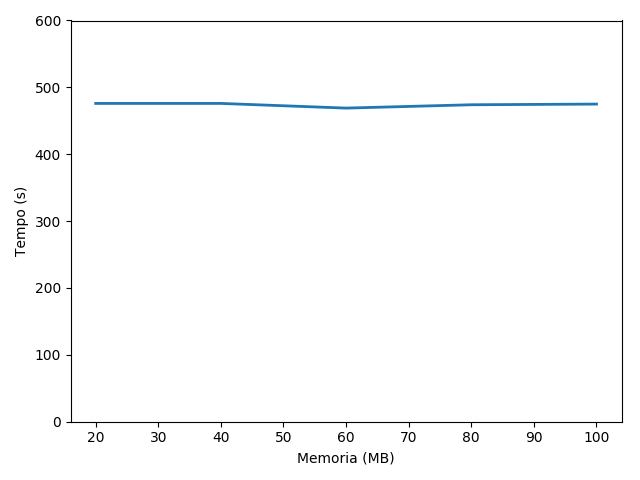
\includegraphics[width=0.6\textwidth]{memoria}
\end{figure}

\section{Melhorias}
Para o uso do indexador implementado em situações reais, deveria haver remoção de acentos nos termos da coleção. Isso diminuiria a quantidade de termos indexados e melhoraria a qualidade das recuperações com o índice. 

O controle de memória pecou, por não ter sido feito de forma estrita e sim com estimativas de consumo de memória por tupla. Isso resultou em usos descontrolados de memória o que impede o uso do indexador para coleções realmente grandes.

%%% End document
\end{document}